\documentclass[a4paper,12pt]{article}
\usepackage[utf8]{inputenc}
\usepackage[spanish]{babel}
\usepackage{color}
\usepackage{parskip}
\usepackage{graphicx}
\usepackage{multirow}
\usepackage{listings}
\usepackage{vmargin}
\usepackage{datetime}
\newdate{date}{12}{10}{2017}
\graphicspath{ {imagenes/} }
\definecolor{mygreen}{rgb}{0,0.6,0}
\definecolor{lbcolor}{rgb}{0.9,0.9,0.9}
\usepackage{epstopdf}
\usepackage{float}


\setpapersize{A4}
\setmargins{2.5cm}       % margen izquierdo
{1.5cm}                        % margen superior
{16.5cm}                      % anchura del texto
{23.42cm}                    % altura del texto
{10pt}                           % altura de los encabezados
{1cm}                           % espacio entre el texto y los encabezados
{0pt}                             % altura del pie de página
{2cm}     

\lstset{
%backgroundcolor=\color{lbcolor},
    tabsize=4,    
%   rulecolor=,
    language=[GNU]C++,
        basicstyle=\tiny,
        aboveskip={1.5\baselineskip},
        columns=fixed,
        showstringspaces=false,
        extendedchars=false,
        breaklines=true,
        prebreak = \raisebox{0ex}[0ex][0ex]{\ensuremath{\hookleftarrow}},
        frame=single,
        showtabs=false,
        showspaces=false,
        showstringspaces=false,
        identifierstyle=\ttfamily,
        keywordstyle=\color[rgb]{0,0,1},
        commentstyle=\color[rgb]{0.026,0.112,0.095},
        stringstyle=\color{red},
        numberstyle=\color[rgb]{0.205, 0.142, 0.73},
%        \lstdefinestyle{C++}{language=C++,style=numbers}’.
}


\begin{document}
\title{Tarea sobre fases y herramientas en la construcción de un compilador}
\author{
Christofer Fabián Chávez Carazas \\
\small{Universidad Nacional de San Agustín de Arequipa} \\
\small{Escuela Profesional de Ciencia de la Computación} \\
\small{Compiladores}
}
\date{\displaydate{date}}

\maketitle

\begin{enumerate}
 \item \textbf{Ejemplificar cada una de las fases en la construcción de un compilador}
 
 \begin{itemize}
  \item \textbf{Analizador Léxico:} El analizador léxico recibe como entrada el código a compilar y produce una
  salida compuesta de tokens. Un token es una cadena de caracteres y son los elementos más básicos sobre los cuales
  se desarrolla toda traducción de un programa. Se describen por lo general en dos partes, una clase y un valor. \\
  Para ejemplificar esta fase, supongamos que tenemos la siguiente línea de código:
  $$WHILE\:contador\:<\:maximo\:THEN$$
  Se pueden identificar los siguientes tokens:
  \begin{itemize}
   \item $[Palabra\:Reservada,``WHILE"]$
   \item $[Identificador,``contador"]$
   \item $[Oerador,``<"]$
   \item $[Identificador, ``maximo"]$
   \item $[Palabra\:Reservada,``THEN"]$
  \end{itemize}

  \item \textbf{Analizador Sintáctico:} El analizador sintáctico recibe como entrada los tokens generados por el
  analizador léxico, y genera un árbol de sintaxis para verificar que los tokens forman una expresión válida. Cada
  nodo del árbol denota una construcción que ocurre en el código fuente. \\
  Para ejemplificar esta fase, extenderemos el seudocódigo anterior:
  $$WHILE\:contador\:<\:maximo\:THEN\:contador=contador + 1\:END$$
  El árbol de sintaxis que se generaría es el siguiente:
  \begin{figure}[H]
   \centering
   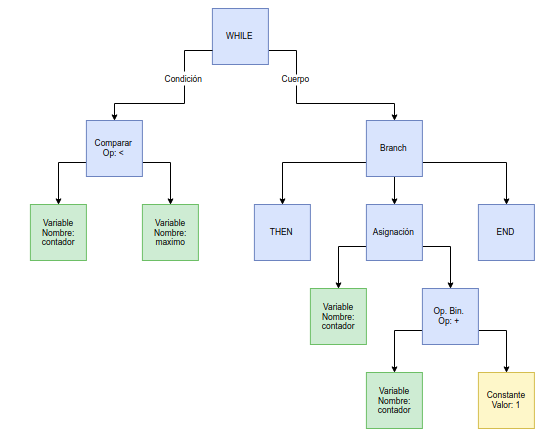
\includegraphics[scale = 0.6]{1.png}
  \end{figure}
  
  \item \textbf{Analizador Semántico:} El analizador semántico recibe como entrada el árbol de sintaxis generado por el
  analizador sintáctico para completar restricciones de tipo y otras limitaciones semánticas, y preparar la generación
  de código. \\
  Para ejemplificar esta fase, supongamos que tenemos el siguiente código;
  \begin{lstlisting}
  int a,b,c,d;
  d = a / (b + c);
  \end{lstlisting}
  En la imagen que sigue, el árbol de la izquierda es generado por el analizador sintáctico, y éste árbol es rellenado por
  el analizador semántico para generar el árbol de la derecha. Esto se genera de forma recursiva.
  \begin{figure}[H]
   \centering
   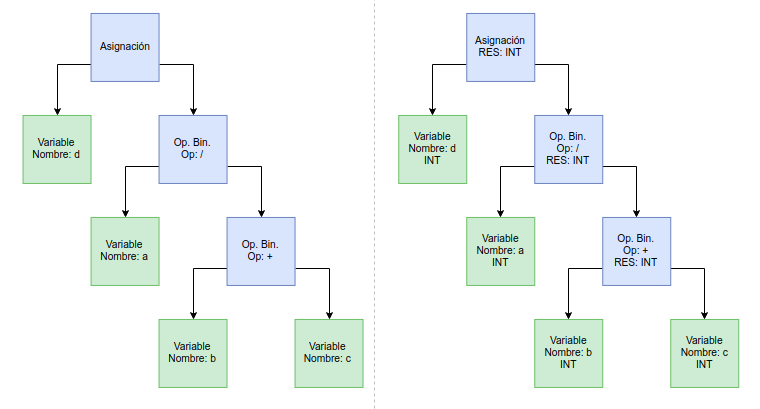
\includegraphics[scale = 0.5]{2.png}
  \end{figure}
  
  \item \textbf{Generador de código intermedio: } El generador de código intermedio recibe como entrada el árbol de sintaxis anotado generado
  por el analizador semántico. La forma más común de expresar el código intermedio es el código de tres direcciones. Éste consiste en una secuencia
  de instrucciones, cada una de las cuales tiene como máximo tres operandos. \\
  Para ejemplificar esta fase, tomaremos la expresión anterior:
  $$d = a / (b + c)$$
  El código de tres direcciones generado es el siguiente:
  \begin{lstlisting}
  r1 = b + c;
  r2 = a / r1;
  d = r2;
  \end{lstlisting}
  
  \item \textbf{Optimizador:}  La finalidad de la optimización de código es producir un código objeto lo más eficiente posible. 
  Revisa el código generado a varios niveles de abstracción y realiza las optimizaciones aplicables al nivel de abstracción.
  Un ejemplo pequeño de una optimización de código es el siguiente:
  \begin{lstlisting}
  do
  {
    item = 10;
    value = value + item; 
  } while(value<100);
  \end{lstlisting}
  \begin{lstlisting}
  item = 10;
  do
  {
    value = value + item; 
  } while(value<100);
  \end{lstlisting}
  
  Se cambia la posición de la instrucción \textbf{item = 10} fuera del bucle, porque en cada iteración se hace una asignación, esto significa que se harían
  100 asignaciones. Al sacarlo fuera del bucle, sólo se hace una asignación.
  
  \item \textbf{Generador de código objeto:} Es la fase final de un compilador, que por lo general consiste en generar código de máquina o código ensamblador.
  Para ejemplificar esta fase, supongamos que tenemos el siguiente código de tres direcciones:
  $$x = y + z$$
  El código ensamblador resultante sería el siguiente:
  \begin{lstlisting}
   MOV y, R0
   ADD z, R0
   MOV R0, x
  \end{lstlisting}

  \item \textbf{Tabla de símbolos:} Es una estructura de datos donde se guardan los símbolos de un código fuente y su información como la ubicación, tipo de datos
  y su ámbito. La tabla de símbolos puede ser usada en todas las fases del compilador. Una forma de guardar las entradas de una tabla de símbolos es la siguiente:
  $$<Nombre\:del\:simbolo,tipo,atributo>$$
  Siguiendo esta estructura, supongamos que tenemos la siguiente declaración.
  \begin{lstlisting}
  static int numero;
  \end{lstlisting}
  Esta variable se debería guardar en la tabla de la siguiente manera:
  $$<numero,int,static>$$

  \item \textbf{Gestión de Errores:} Recibe el código de error cuando en el análisis se detecta un error, y se encarga de escribir un mensaje con el error
  correspondiente, así como cortar el proceso de traducción. Dependiendo de en qué fase se de el error pueden ser errores léxicos, errores sintácticos y 
  errores semánticos. Un pequeño ejemplo sería cuando en el código existen caracteres inválidos.
 \end{itemize}

 \item \textbf{Indagar e investigar sobre herramientas para la construcción de compiladores}
 
 \begin{itemize}
  \item \textbf{Bison:} Es un generador de analizadores sintácticos de propósito general que convierte una descripción gramatical para una gramática independiente del contexto en un programa en C que analice esa gramática. Es utilizado en un amplio rango de analizadores de lenguajes, desde aquellos usados en simples calculadoras de escritorio hasta complejos lenguajes de programación.
  \item \textbf{Lex:} Es un generador de analizador léxico, que sirve para generar los token para la siguiente fase . La principal característica de Lex es que va a permitir asociar acciones descritas en C, a la localización de las Expresiones Regulares que se hayan definido. Para ello Lex se apoya en una plantilla que recibe como parámetro, y que se debe diseñar con cuidado. Internamente Lex va a actuar como un autómata que localizará las expresiones regulares que se le describan, y una vez reconocida la cadena representada por dicha expresión regular, ejecutará el código asociado a esa regla.
  \item \textbf{Yacc:} Es un programa para generar analizadores sintácticos. Las siglas del nombre significan Yet Another Compiler Compiler, es decir, "Otro generador de compiladores más". Genera un analizador sintáctico (la parte de un compilador que comprueba que la estructura del código fuente se ajusta a la especificación sintáctica del lenguaje) basado en una gramática analítica.Yacc genera el código para el analizador sintáctico en el Lenguaje de programación C.
  \item \textbf{Flex:} Es una herramienta para generar escáneres: programas que reconocen patrones léxicos en un texto. Flex lee los ficheros de entrada dados, o la entrada estándar si no se le ha indicado ningún nombre de fichero, con la descripción de un escáner a generar. Estas herramientas de apoyo han sido reescritas para otros lenguajes, incluyendo Ratfor, EFL, ML,Ada, Java, Python, y Limbo. De esta forma se ha logrado una mayor utilización de las mismas en diferentes compiladores desarrollados sobre tecnologías libres. Teniendo en cuenta las características de las aplicaciones antes mencionadas, se ha escogido para la realización del compilador las herramientas Yacc y Lex. En muchos de los compiladores desarrollados en el mundo suelen ser utilizados juntos. Yacc utiliza una gramática formal para analizar un flujo de entradas, algo que Lex no puede hacer con expresiones regulares simples (Lex se limita a los autómatas de estados finitos simples). Sin embargo, Yacc no puede leer en un flujo de entradas simple, requiere una serie de símbolos. Lex se utiliza a menudo para proporcionar a Yacc estos símbolos.
 \end{itemize}

 
 
\end{enumerate}


\end{document}

